\documentclass{scrartcl}
\usepackage{german}
\usepackage[T1]{fontenc}
\usepackage[latin1]{inputenc}
\usepackage[german]{babel}

% zusätzliche mathematische Symbole, AMS=American Mathematical Society
\usepackage{amssymb}

% fürs Einbinden von Graphiken
\usepackage{graphicx}

% für Namen etc. in Kopf- oder Fußzeile
\usepackage{fancyhdr}

% erlaubt benutzerdefinierte Kopfzeilen
\pagestyle{fancy}

% Definition der Kopfzeile
\lhead{
\begin{tabular}{ll}
Fisnik Zeqiri & 4306430 \\
Felix  Karg   & 4342014
\end{tabular}
}
\chead{}
\rhead{\today{}}
\lfoot{}
\cfoot{Seite \thepage}
\rfoot{}

\begin{document}
\section*{Antworten zum �bungsblatt Nr. 9}

\section*{Aufgabe 1}
    \begin{itemize}
        \item[a)] 
            x -> y: [0.01:0.15]; y -> z: [0.00:0.08] (0 -> 0) \\
            x -> y: [0.00:0.08]; y -> z: [0.01:0.15] (1 -> 1) \\
            maximale Zeit: 0.08 + 0.15 = 0.23 [ns].
        \item[b)] [Bild 1] [Bild 2] \\
                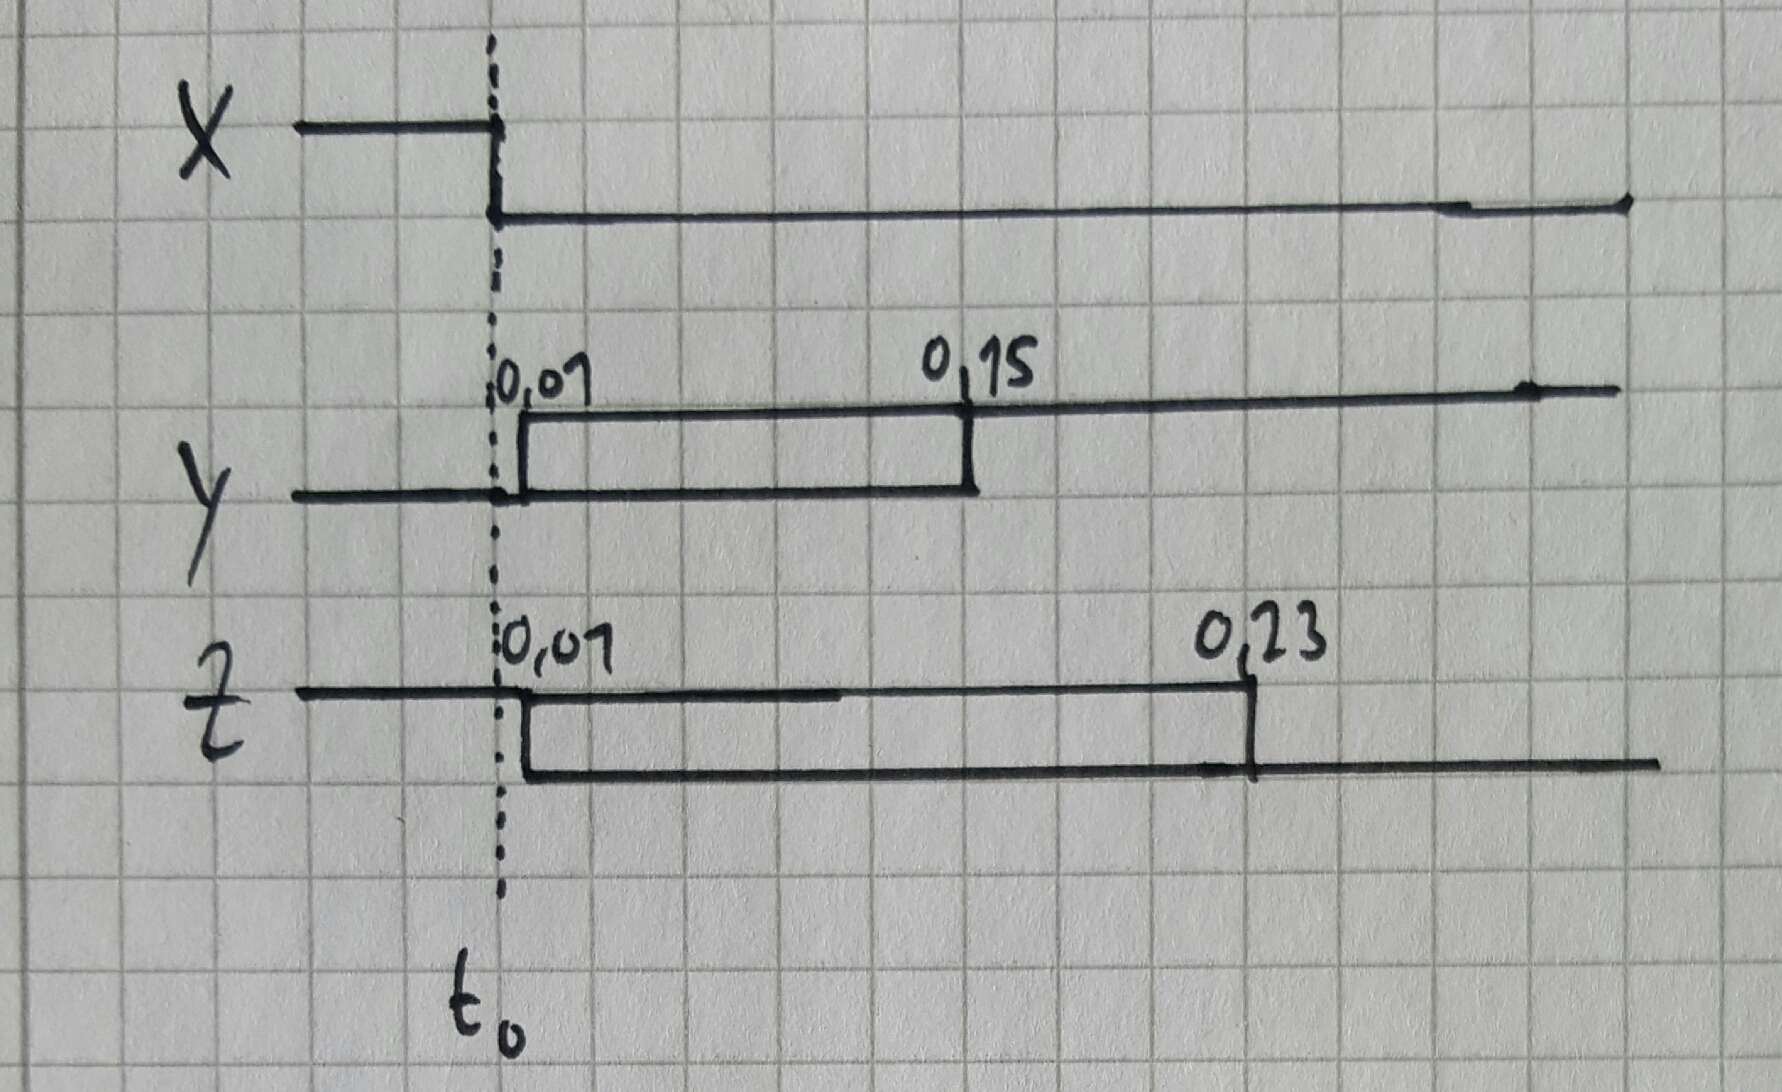
\includegraphics[width=7cm]{20161219_135856.jpg}
                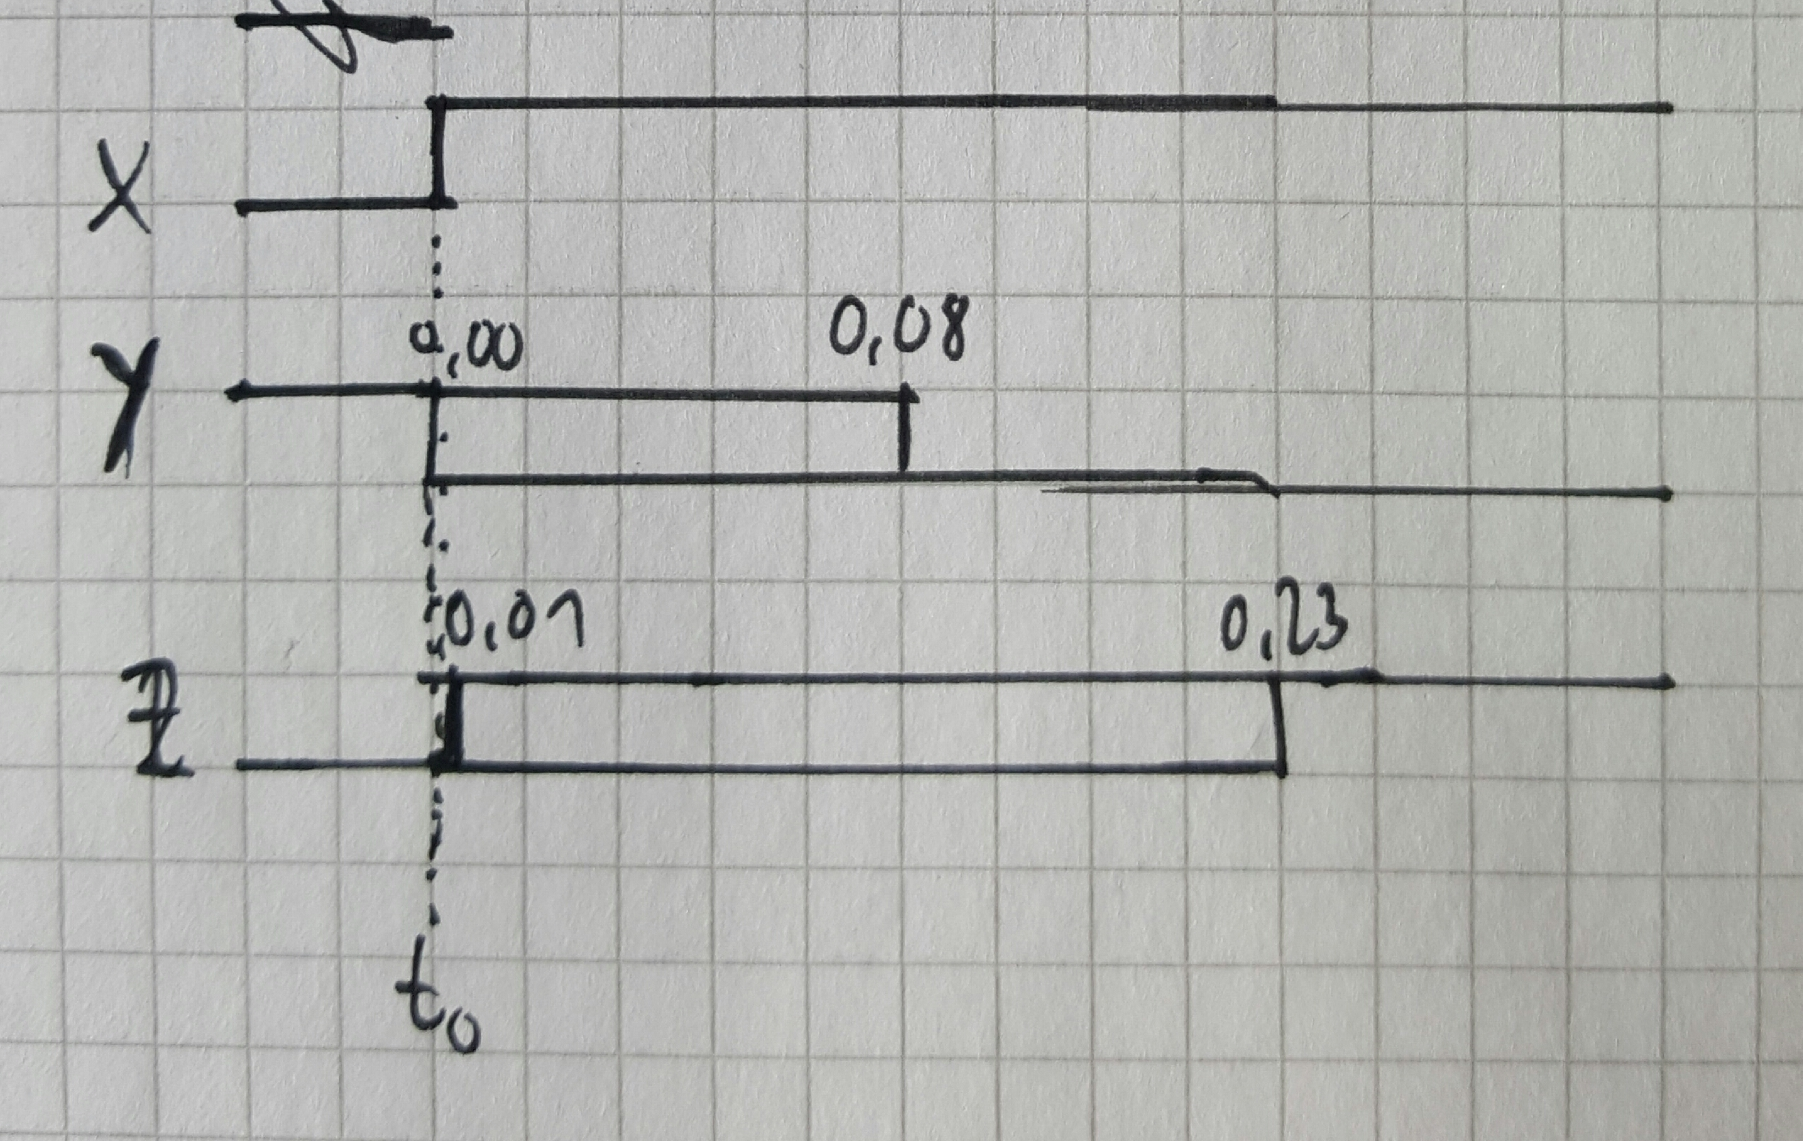
\includegraphics[width=7cm]{20161219_135918.jpg} \\
            -> Immer zwischen [0.01:0.15] + [0.00:0.08] = 
                [0.01:0.15] + [0.00:0.08] = [0.01:0.23].
    \end{itemize}

\section*{Aufgabe 2}
\begin{verbatim}
x = 0 -> 1
a = 1 -> 0
b = c = 0 -> 1
d = e = 1 -> 0
f = [0.02:0.14] + [0.01:0.07] + [0.02:0.14] = [0.07:0.35] (1 -> 0)
g = [0.02:0.14] + [0.01:0.07] + [0.02:0.14] = [0.07:0.35] (1 -> 0)
h = [0.02:0.14] + [0.01:0.07]               = [0.03:0.21] (0 -> 1)
i = [0.02:0.14] + [0.01:0.07] + [0.02:0.07] = [0.05:0.28] (0 -> 1)
j = [0.02:0.14]                             = [0.02:0.14] (1 -> 0)
k = [0.02:0.14] + [0.03:0.10] + [0.01:0.07] = [0.06:0.31] (0 -> 1)
l = [0.02:0.14] + [0.03:0.10]               = [0.05:0.24] (1 -> 0)
m = [0.02:0.14] + [0.03:0.10] + [0.03:0.10] = [0.08:0.34] (1 -> 0)
n = [0.02:0.14] + [0.03:0.10] + [0.03:0.10] = [0.08:0.34] (1 -> 0)

o = [max(min(f..n)):max(f..n)]+ [0.05:0.15] = [0.13:0.50] (0 -> 1)
p = [0.13:0.50] + [0.01:0.07]               = [0.14:0.57] (1 -> 0)

\end{verbatim}
Bei Ausgang o und genauso bei p kann sogar ab 0.06 bzw 0.07 ns das korrekte
Ergebnis ausgegeben sein, allerdings hatten zu diesem Zeitpunkt definitiv noch
nicht alle gatter die M�glichkeit �berhaupt das korrekte ergebnis zu liefern,
selbst mit Minimalreaktionszeit. \\
Es kann daher bei o und genauso bei p sein, dass bis 0.50 bzw. 0.57 ns
respektive das Ergebnis mehrfach flackert.


\section*{Aufgabe 3}
\begin{itemize}
    \item[a)] Ja, $\delta$ ist $\geq$ der Unterschied von $t_2$ bis $t_4$ 
        (per Definition), also ist $t_2 + \delta \geq t_4$.
    \item[b)] Nein, Da man �ber die verteilung von $\delta/2$ keine genaue
        Aussage treffen kann und im allgemeinen $t_3 < t_4$.
    \item[c)] Ja, folgt transitiv aus $t_3 < t_4$ (-> a).
    \item[d)] Ja, da $t_2 \leq t_3$ immer gilt.
    \item[e)] Nein, siehe b.
    \item[f)] Nur, falls $\delta \geq t_p$
    \item[g)] Nein, Da $t_2 < t_3$, aber $t_3$ ben�tigt w�re. (~1 $\delta$)
    \item[h)] Ja, da $(t_8 - t_3) = t_p$, sowie $t_p + 2 * \delta$ ein ganzer
        Spannungsverlauf ist, welcher alleine schon mindestens gleich $t_{10}$
        ist.
\end{itemize}

\section*{Aufgabe 4}
$t_{HWD}$ ergibt sich dadurch, dass das NAND-Gatter spikefrei umschalten muss,
wof�r es nach dem Absenken von $W$ noch 0.41 [ns] ben�tigt, damit $D$ ohne sorgen
umgeschaltet werden kann.
\\
\\
$t_{SWD}$ ist genau das umschalten eines NANDs plus die umschaltzeit des eines
NOT-Gatters vor dem /R-NAND, die Volle Zeit wird aber nur ben�tigt, sollte D
zuvor $0$ gewesen sein (somit das Not noch bis zu 8ns lang 1, und um den neuen 
Wert zu spikefrei zu schreiben, ben�tigt das NAND au�erdem noch 41ns -> 49ns).
\\
\\
Die Zeit f�r $y$ setzt sich ein wenig komplizierter zusammen. Und zwar wie folgt:\\
Wenn $W$ 'kommt', dann braucht ein NAND zwischen [0.01:0.12]ns, um richtig
zu schalten. Unser RS-FF ben�tigt eine Pulsweite von mindestens 0.68ns um das
richtige abzuspeichern. Beim Umschalten danach ben�tigt das selbe NAND wieder
mindestens 0.01 ns, weswegen unser FF nun insgesamt 0.69ns bekommen hat.
Addieren wir also nur 0.67ns zu den maximalen 0.12 des NANDs, kommen wir auf
0.79ns, wobei das RS-FF immernoch 0.68ns Zeit hat -> $y = 0.79ns$.


\section*{Aufgabe 5}
    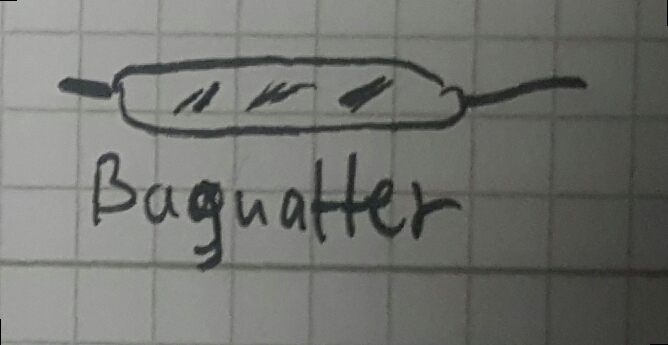
\includegraphics[width=7cm]{20161221_143637.jpg}
    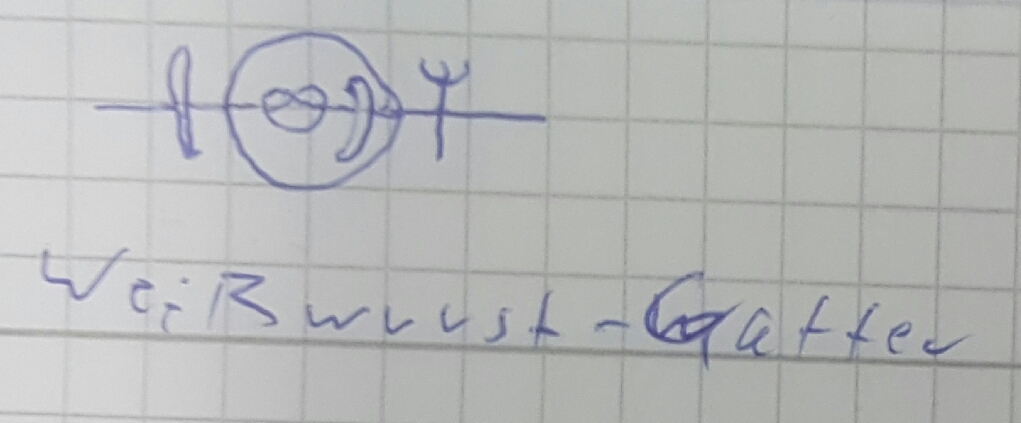
\includegraphics[width=7cm]{20161221_143548.jpg} \\
    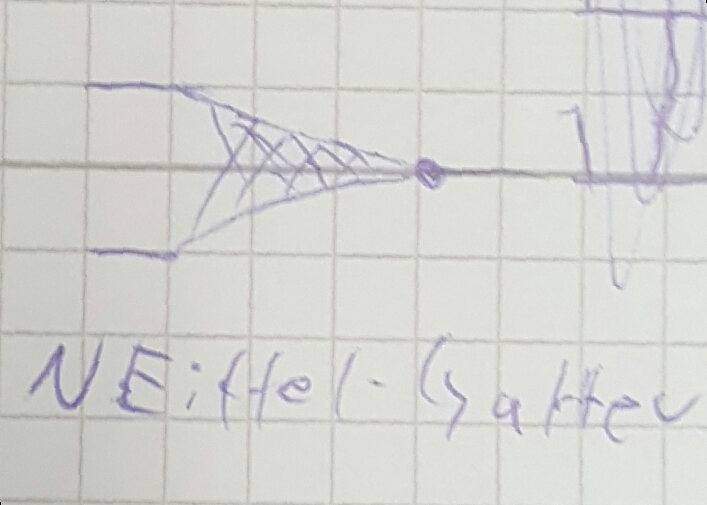
\includegraphics[width=7cm]{20161221_143351.jpg}
    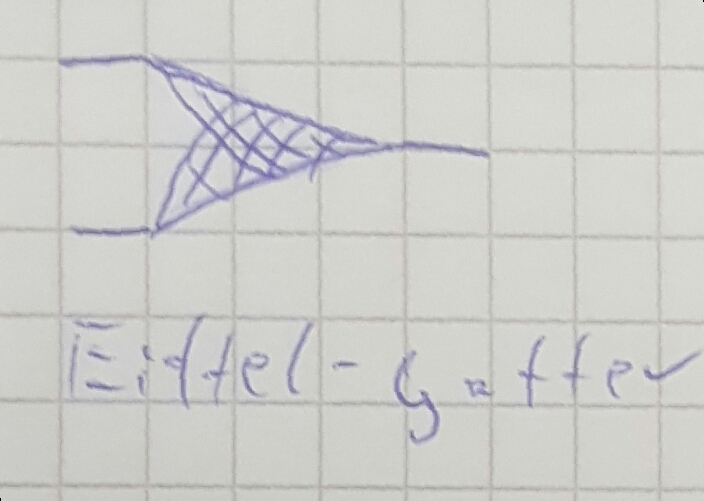
\includegraphics[width=7cm]{20161221_143327.jpg} \\
    Baguatter: Man lege ein unger�stes Baguett hinein und nach gewisser zeit ist es fertig :) \\
    Wei�wurst-Gatter: Mann nehme ein gutes Bayrisches Bier -> Mahlzeit. \\
    Eiffel-Gatter: F�hrt zwei Teilschaltkreise auf Elegante Art und Weise zusammen. \\
    NEiffel-Gatter: negiertes Eiffel-Gatter




\end{document}

